% vim: set spell spelllang=es syntax=tex :

\documentclass[11pt,a4paper,spanish]{beamer}

\usepackage[spanish]{babel}

\usepackage[utf8]{inputenc}

\usepackage{graphicx}

\usepackage{subcaption} %Para Subfigure

\usepackage{caption} %Para captions en las figuras sin prefijo

\usepackage{ccicons}

\usepackage{url}

\usepackage{babelbib}

\usepackage{textcomp}
\newcommand{\aprox}{\raisebox{0.5ex}{\texttildelow}}

\usefonttheme{serif}

\setlength{\parskip}{1.5mm}

\usetheme{Rochester}
\usecolortheme{whale}

%\usetheme{Warsaw}

\beamertemplatenavigationsymbolsempty

\setbeamertemplate{background canvas}{
    \raisebox{-0.99\paperheight}[0pt][0pt]{
        \makebox[\paperwidth]{
            \null
            \hspace{-1em}
            
\includegraphics[width=0.09\paperwidth]{logos/fai.pdf}
            \hspace{0.8\paperwidth}
            \hspace{-0.5em}
            \includegraphics[width=0.09\paperwidth]{logos/uncoma.pdf}
            }
    }
}

\title{Historia de los sistemas de computo}

\author{}

\date{}

\defbeamertemplate{footline}{centered page number}
{
    \hspace*{\fill}
    \usebeamercolor[fg]{blue}
    \usebeamerfont{page number in head/foot}
    \insertpagenumber\,/\,\insertpresentationendpage
    \hspace*{\fill}\vskip2pt
}
\setbeamertemplate{footline}[centered page number]

\begin{document}

\begin{frame}[noframenumbering]

    \maketitle
    \centering
    \vspace{-8em}~
    \begin{figure}
    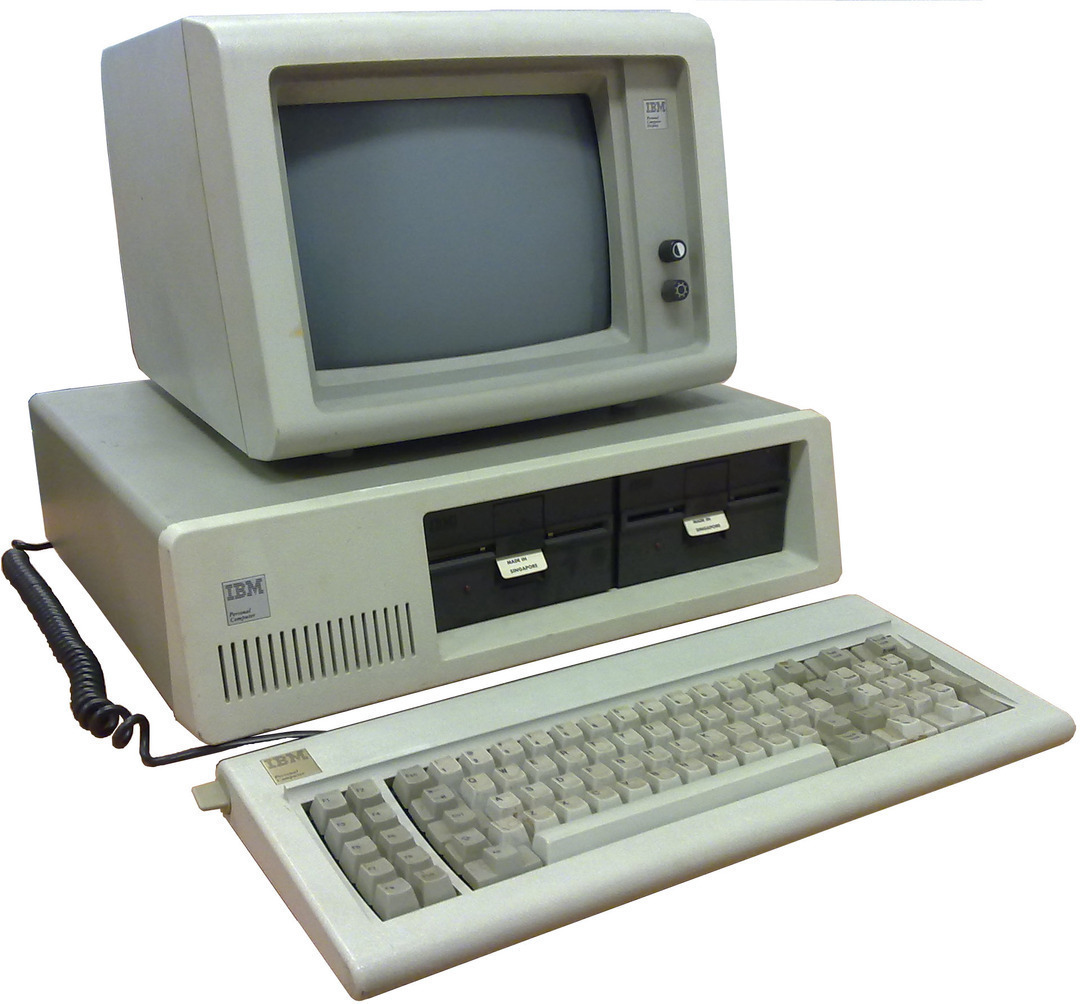
\includegraphics[height=0.65\textheight]{img/ibm-pc-5150.jpg}
        \captionsetup{textfont=tiny,labelformat=empty}
        \caption{IBM PC 5150 \ccbysa\cite{ibm-pc-5150}}
    \end{figure}

\end{frame}

\begin{frame}

    \frametitle{Temario}

\begin{enumerate}

    \setcounter{enumi}{-1}

    \item Antecedentes históricos.

    \item Primera generación: válvulas de vacío.

    \item Segunda generación: Transistores.

    \item Tercera generación: Circuitos integrados.

    \item Cuarta generación: Integración a gran escala.

\end{enumerate}

\end{frame}

\begin{frame}

\frametitle{Antecedentes históricos}
\framesubtitle{El mecanismo de Anticitera ({\aprox}150 a.e.c)}


\begin{itemize}
    \item La computadora mecánica más antigua conocida.
    \item Aparentemente podía calcular las posiciones de los astros.
    \item Una única tarea.
\end{itemize}


    \begin{figure}
        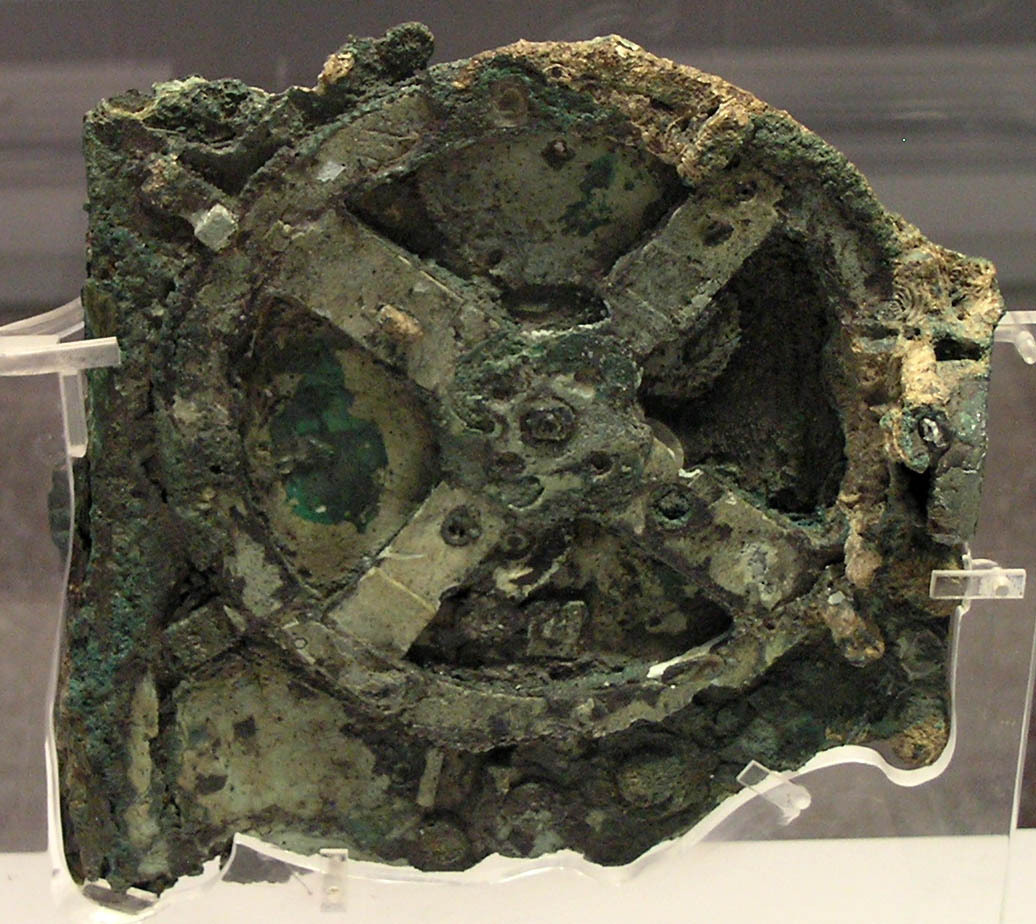
\includegraphics[width=0.5\textwidth]{img/anticitera.jpg}
        \captionsetup{textfont=tiny,labelformat=empty}
        \caption{\ccbysa\cite{anticitera}}
    \end{figure}


\end{frame}

\begin{frame}

\frametitle{Antecedentes históricos}
\framesubtitle{Máquina analítica de Charles Babbage (1837)}

\begin{minipage}{0.2\textwidth}
    \centering
    \begin{figure}
        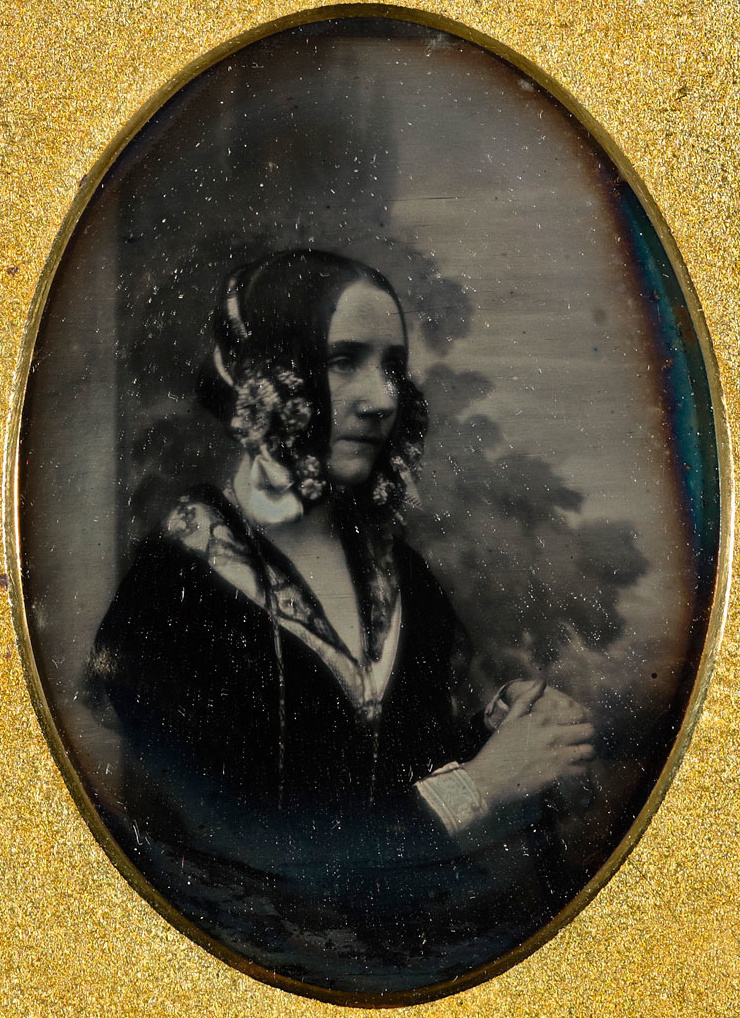
\includegraphics[width=1.0\textwidth]{img/ada.jpg}
        \captionsetup{textfont=tiny,labelformat=empty}
        \caption{Ada Lovelace}
    \end{figure}
\end{minipage}
~
\begin{minipage}{0.55\textwidth}
    \centering
    \begin{itemize}
        \item ¡Primera computadora de propósito general!
        \item Se programaba utilizando tarjetas perforadas.
        \item Nunca fue construida.
    \end{itemize}
\end{minipage}
~
\begin{minipage}{0.2\textwidth}
    \centering
    \begin{figure}
        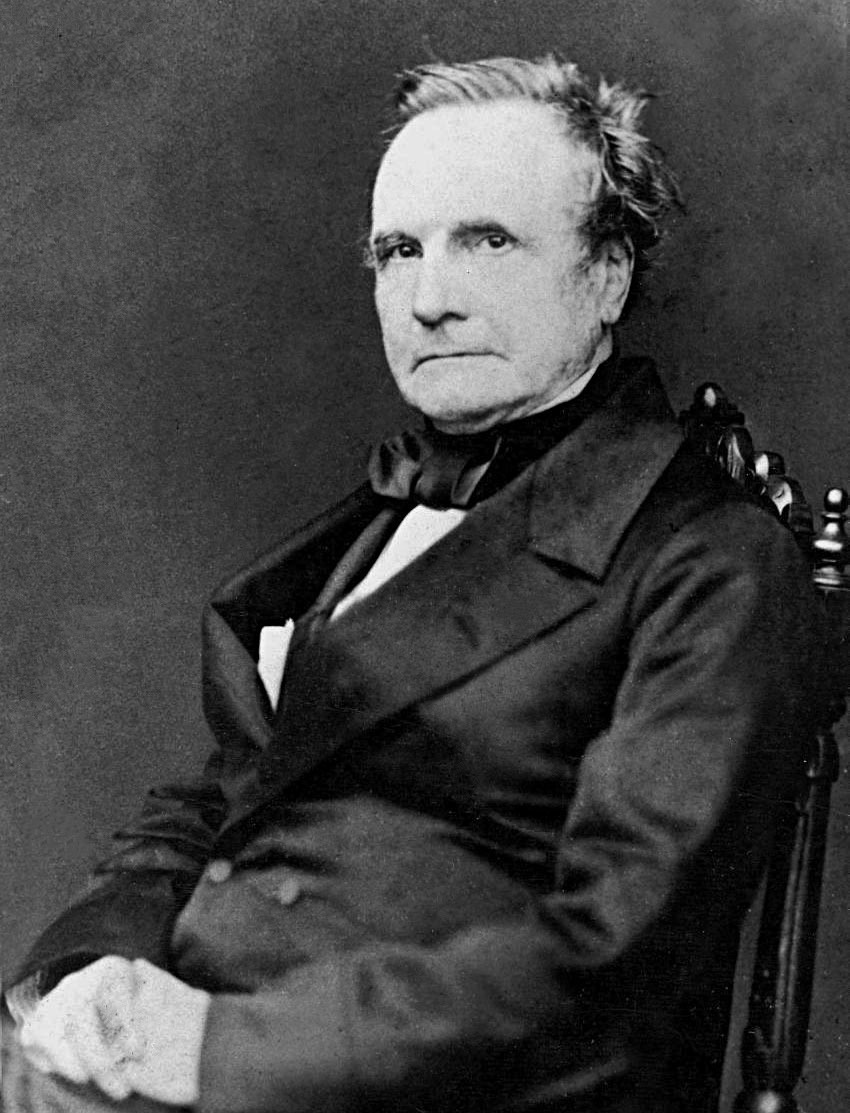
\includegraphics[width=1.0\textwidth]{img/babbage.jpg}
        \captionsetup{textfont=tiny,labelformat=empty}
        \caption{Charles Babbage}
    \end{figure}
\end{minipage}

\end{frame}

\begin{frame}

\frametitle{Antecedentes históricos}
\framesubtitle{La máquina tabuladora de Hollerith (1890)}

\begin{minipage}{0.66\textwidth}

    \begin{itemize}
        \item Diseñada para asistir en el censo de EEUU.
        \item Cada tarjeta representa una persona.
        \item Permitió el procesamiento de grandes volúmenes de datos.
        \item Electromecánica.
    \end{itemize}

\end{minipage}
~
\begin{minipage}{0.3\textwidth}

    \begin{figure}
        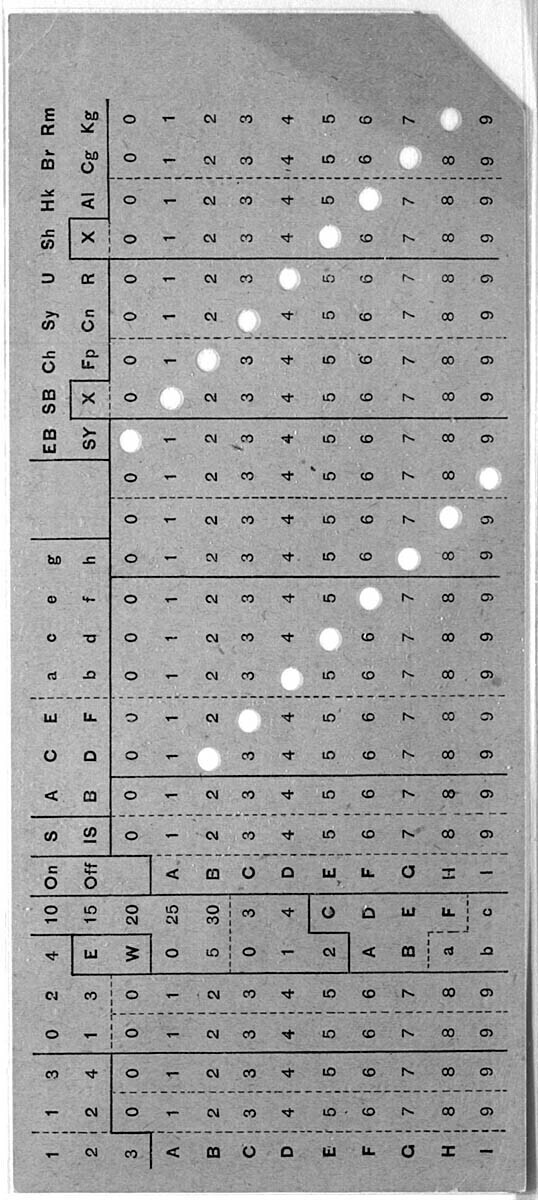
\includegraphics[width=1.0\textwidth]{img/hcard.jpg}
        \captionsetup{textfont=tiny,labelformat=empty}
        \caption{}
    \end{figure}

\end{minipage}

\end{frame}

\begin{frame}

\frametitle{Primera generación}
\framesubtitle{La válvula de vacío}

\begin{minipage}{0.66\textwidth}

    \begin{itemize}
        \item Permite controlar el flujo de electricidad utilizando una señal
            de control.
        \item En conjunto permiten crear compuertas lógicas y memorias de un
            bit.
        \item Consumen mucha energía y tienen una vida útil corta.
    \end{itemize}

\end{minipage}
~
\begin{minipage}{0.3\textwidth}

    \begin{figure}
        
\includegraphics[width=1.0\textwidth]{img/vtube.png}
        \captionsetup{textfont=tiny,labelformat=empty}
        \caption{}
    \end{figure}

\end{minipage}

\end{frame}

\begin{frame}

\frametitle{Primera generación}
\framesubtitle{Colossus (1943, 1944)}


    \begin{itemize}
        \item Primera computadora programable en funcionamiento.
        \item Diseñada con el fin de decodificar mensajes encriptados.
        \item Se programaba activando y desactivando interruptores físicos.
    \end{itemize}


    \begin{figure}
        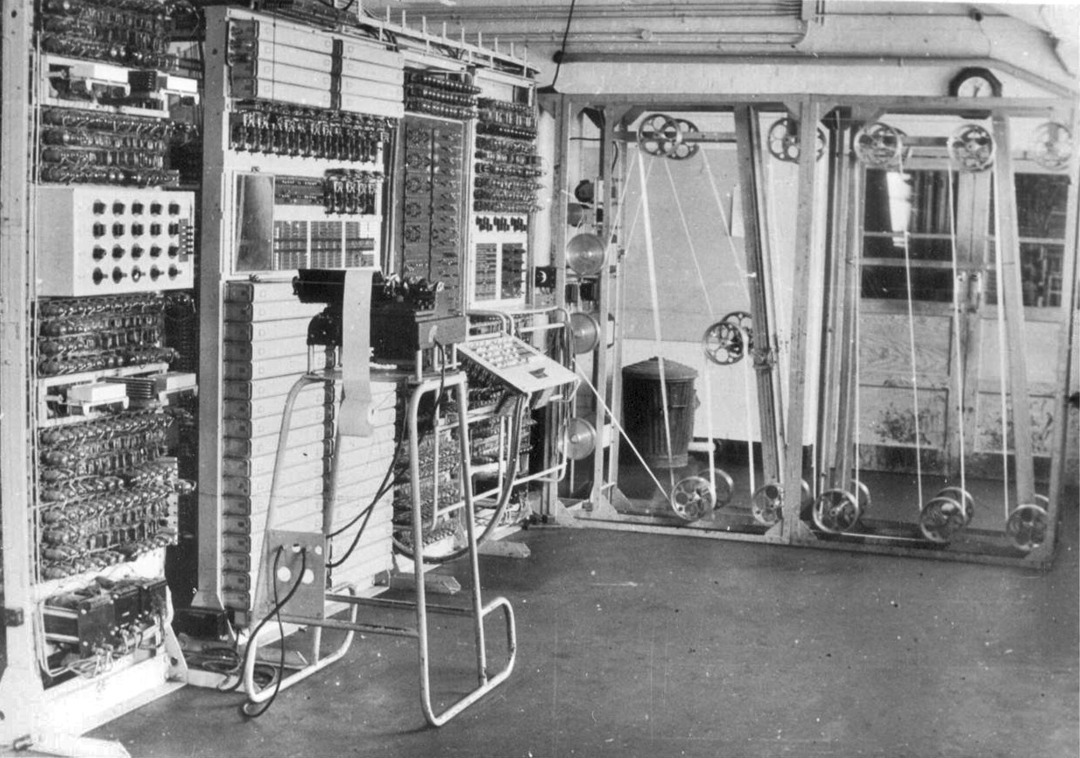
\includegraphics[width=0.5\textwidth]{img/colossus.jpg}
        \captionsetup{textfont=tiny,labelformat=empty}
        \caption{}
    \end{figure}


\end{frame}

\begin{frame}

\frametitle{Primera generación}
\framesubtitle{Colossus (1943, 1944)}

\begin{figure}
    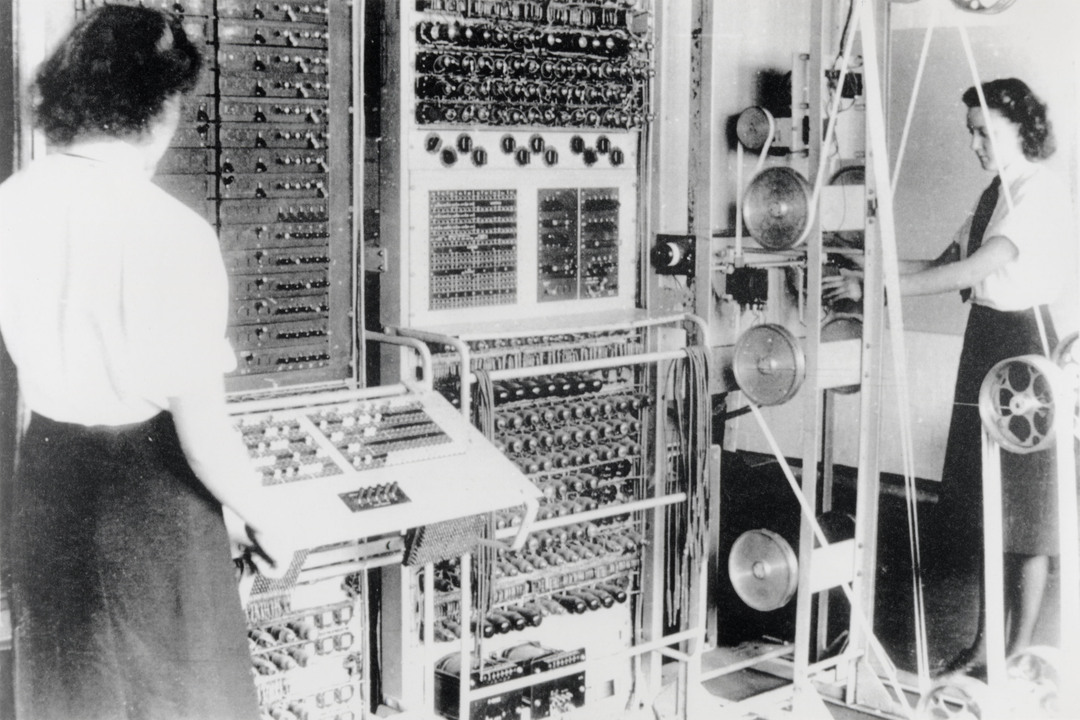
\includegraphics[width=0.9\textwidth]{img/colossus2.jpg}
    \captionsetup{textfont=tiny,labelformat=empty}
    \caption{}
\end{figure}

\end{frame}

\begin{frame}

\frametitle{Primera generación}
\framesubtitle{ENIAC (1945)}


    \begin{itemize}
        \item Propuesta para cómputos de trayectoria de proyectiles:
        \begin{itemize}
            \item $5\,000$ sumas por segundo.
            \item $357$ multiplicaciones por segundo.
            \item Aun así redujo el tiempo de 20 horas a 30 segundos.
        \end{itemize}
        \item Se programaba activando y desactivando interruptores físicos.
    \end{itemize}


    \begin{figure}
        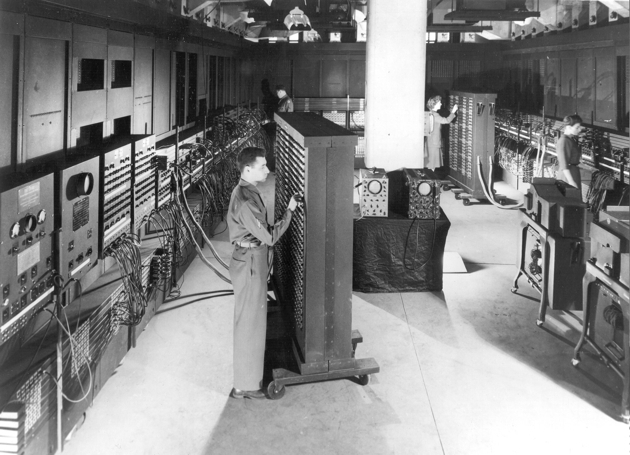
\includegraphics[width=0.5\textwidth]{img/eniac.jpg}
        \captionsetup{textfont=tiny,labelformat=empty}
        \caption{}
    \end{figure}


\end{frame}

\begin{frame}

\frametitle{Primera generación}
\framesubtitle{ENIAC (1945)}

\begin{figure}
    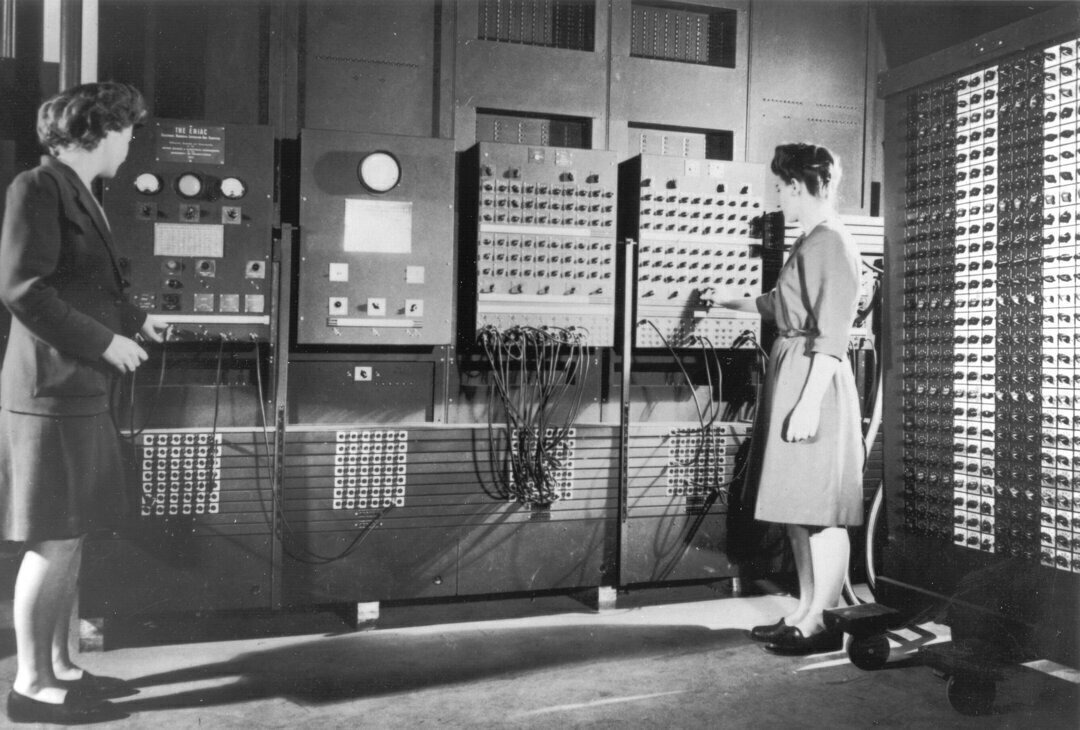
\includegraphics[width=0.9\textwidth]{img/eniac2.jpg}
    \captionsetup{textfont=tiny,labelformat=empty}
    \caption{}
\end{figure}

\end{frame}

\begin{frame}

\frametitle{Primera generación}
\framesubtitle{El bebe de Manchester (1948)}

\begin{itemize}
    \item ¡Primera computadora de programa almacenado!
    \item No tenia una finalidad práctica, pero demostró que el concepto era
        aplicable.
\end{itemize}

\begin{figure}
    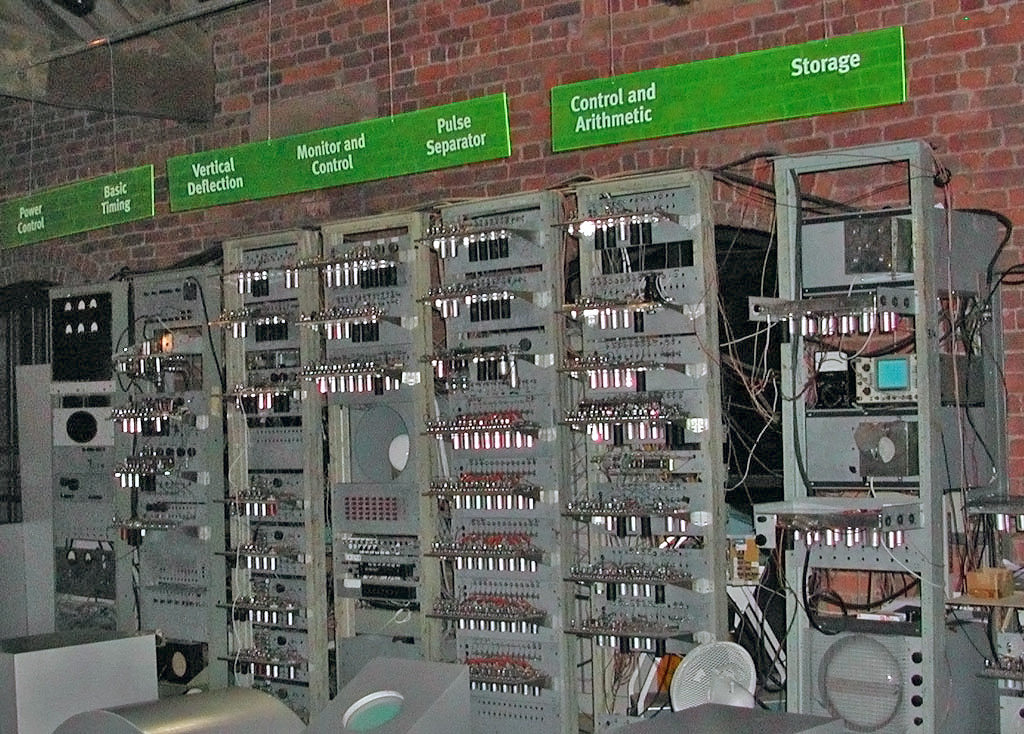
\includegraphics[width=0.5\textwidth]{img/mbaby.jpg}
    \captionsetup{textfont=tiny,labelformat=empty}
    \caption{}
\end{figure}

\end{frame}

\begin{frame}

\frametitle{Segunda generación}
\framesubtitle{El transistor (1947)}

\begin{minipage}{0.66\textwidth}

    \begin{itemize}
        \item Función similar a las válvulas de vacío:
        \begin{itemize}
            \item Menor consumo energético.
                \emph{\tiny{(menos~calor)}}
            \item Más resistentes.
            \item Menor tamaño.
        \end{itemize}
    \end{itemize}

\end{minipage}
~
\begin{minipage}{0.3\textwidth}

    \begin{figure}
        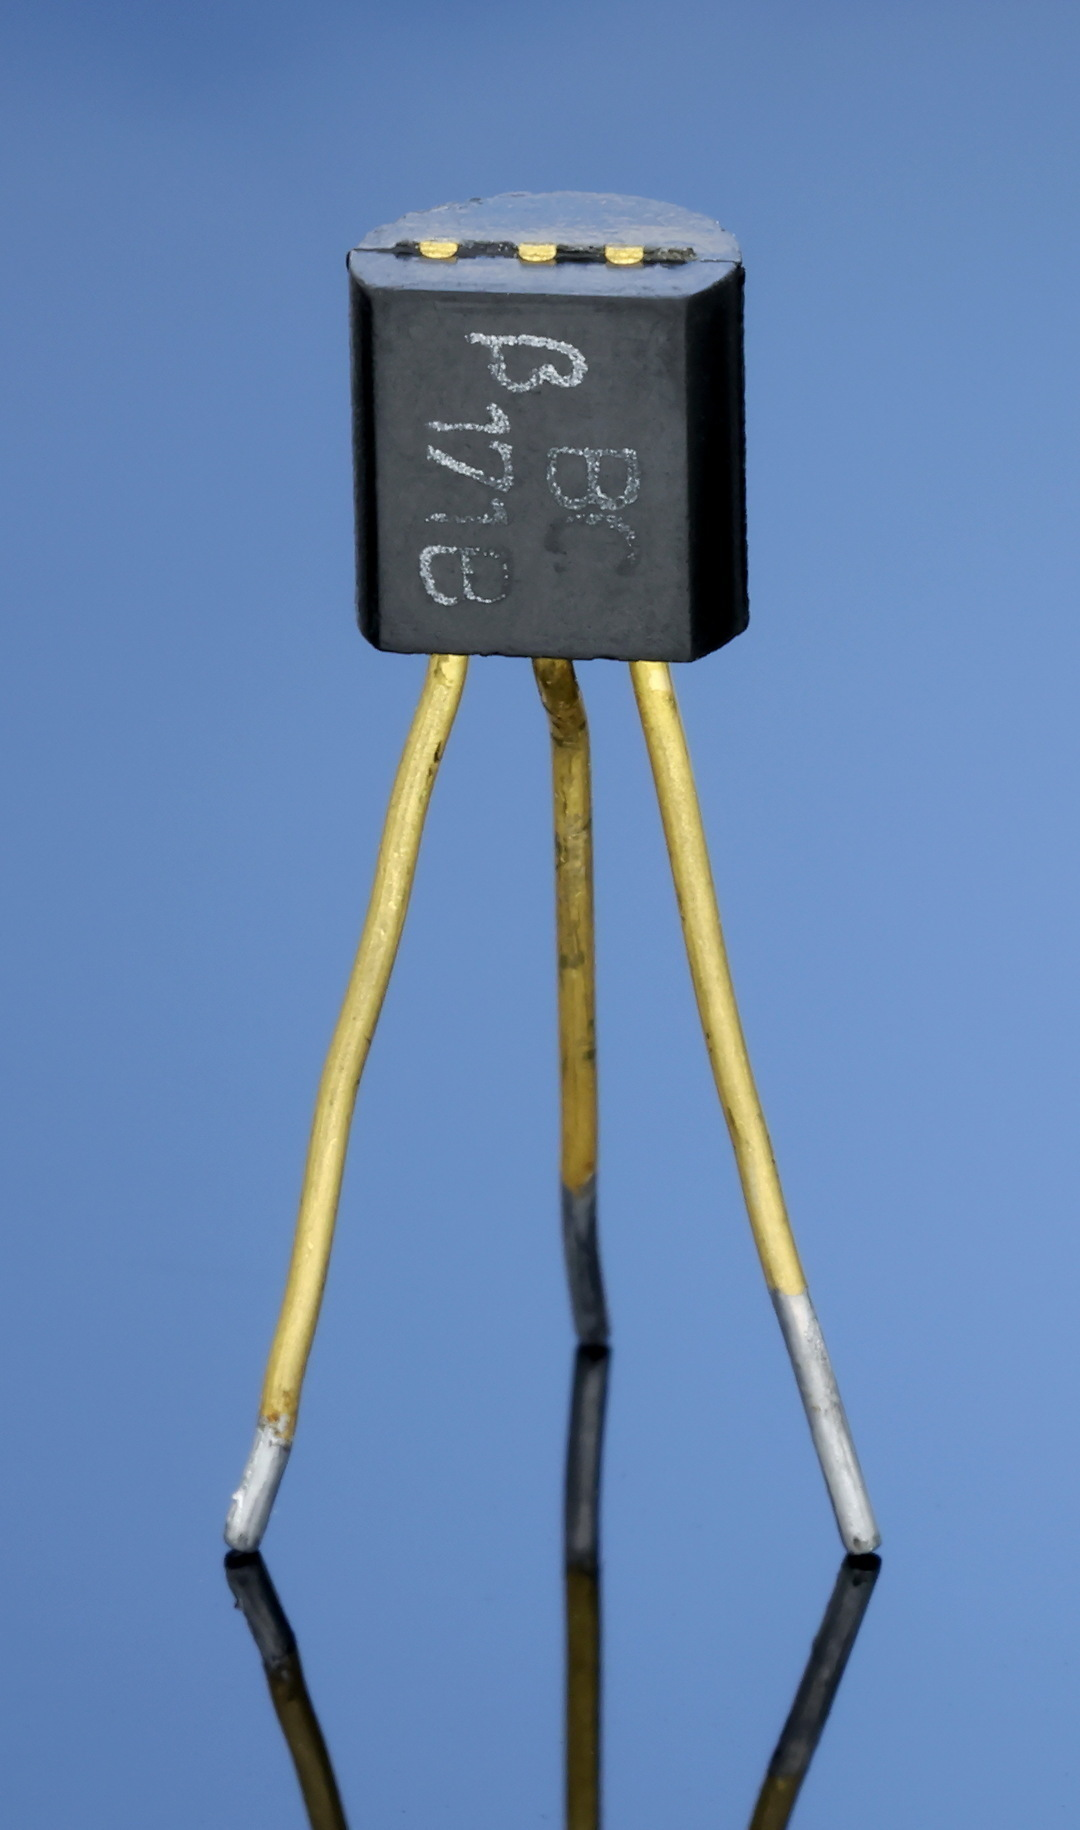
\includegraphics[width=1.0\textwidth]{img/transistor.jpg}
        \captionsetup{textfont=tiny,labelformat=empty}
        \caption{}
    \end{figure}

\end{minipage}

\end{frame}

\begin{frame}

\frametitle{Segunda generación}
\framesubtitle{PDP-1 (1959)}

\begin{figure}
    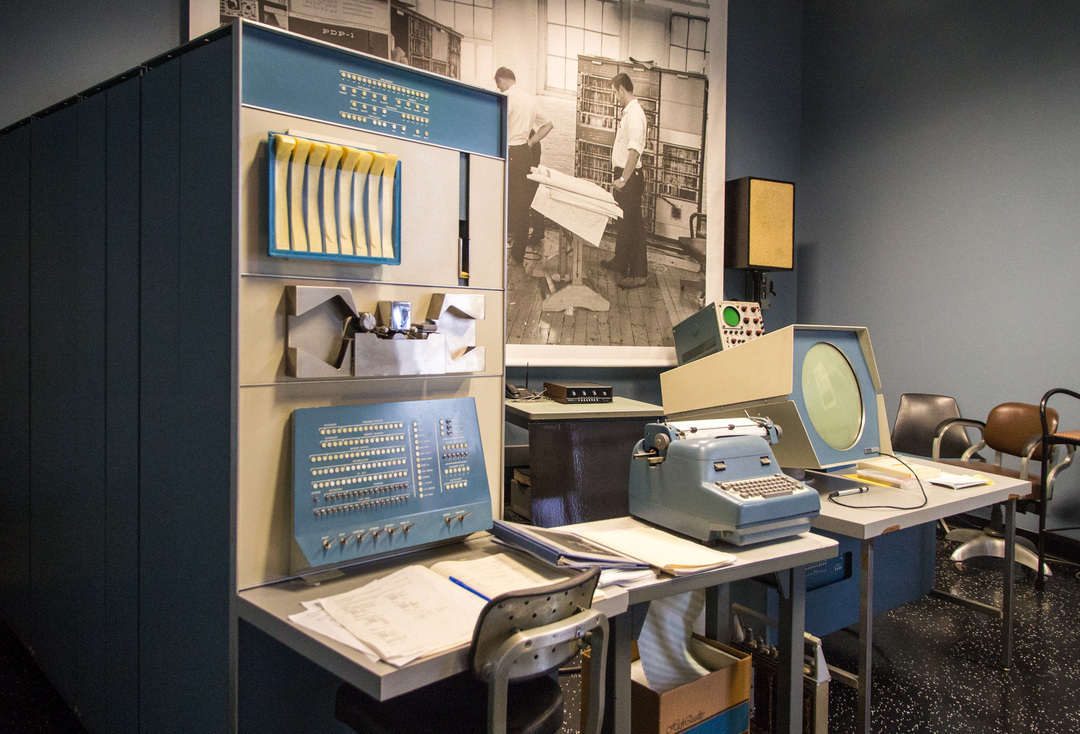
\includegraphics[width=0.9\textwidth]{img/pdp1.jpg}
    \captionsetup{textfont=tiny,labelformat=empty}
    \caption{\ccbysa\cite{pdp1}}
\end{figure}

\end{frame}

\begin{frame}

\frametitle{Tercera generación}
\framesubtitle{Circuitos integrados (1965)}

\begin{minipage}{0.66\textwidth}
\begin{itemize}
    \item Se integran transistores en un sólo componente.
    \item Menor tamaño y costo.
    \item Facilita la abstracción.
\end{itemize}
\end{minipage}
~
\begin{minipage}{0.3\textwidth}
\begin{figure}
    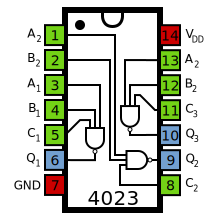
\includegraphics[width=1.0\textwidth]{img/dip-nand.pdf}
    \captionsetup{textfont=tiny,labelformat=empty}
    \caption{}
\end{figure}
\end{minipage}

\end{frame}
\begin{frame}

\frametitle{Cuarta generación}
\framesubtitle{Integración a gran escala (1971)}

\begin{minipage}{0.66\textwidth}
\begin{itemize}
    \item Se integran miles de transistores en un solo componente.
    \item Permite la creación de componentes de alta complejidad:
        \begin{itemize}
            \item Microprocesadores.
            \item Chips de memoria.
            \item \emph{system-on-chip}.
        \end{itemize}
\end{itemize}
\end{minipage}
~
\begin{minipage}{0.3\textwidth}
\begin{figure}
    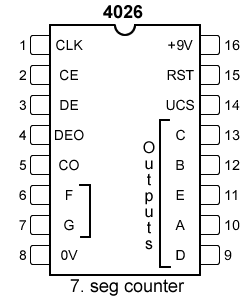
\includegraphics[width=1.0\textwidth]{img/4026-chip.png}
    \captionsetup{textfont=tiny,labelformat=empty}
    \caption{\ccbysa\cite{4026-chip}}
\end{figure}
\end{minipage}

\end{frame}

\begin{frame}

\frametitle{Cuarta generación}
\framesubtitle{Intel 4004 (1971)}

\begin{itemize}
    \item Primer procesador comercial.
    \item Toda la CPU en un solo componente.
    \item $2\,300$ transistores.
\end{itemize}

\begin{figure}
    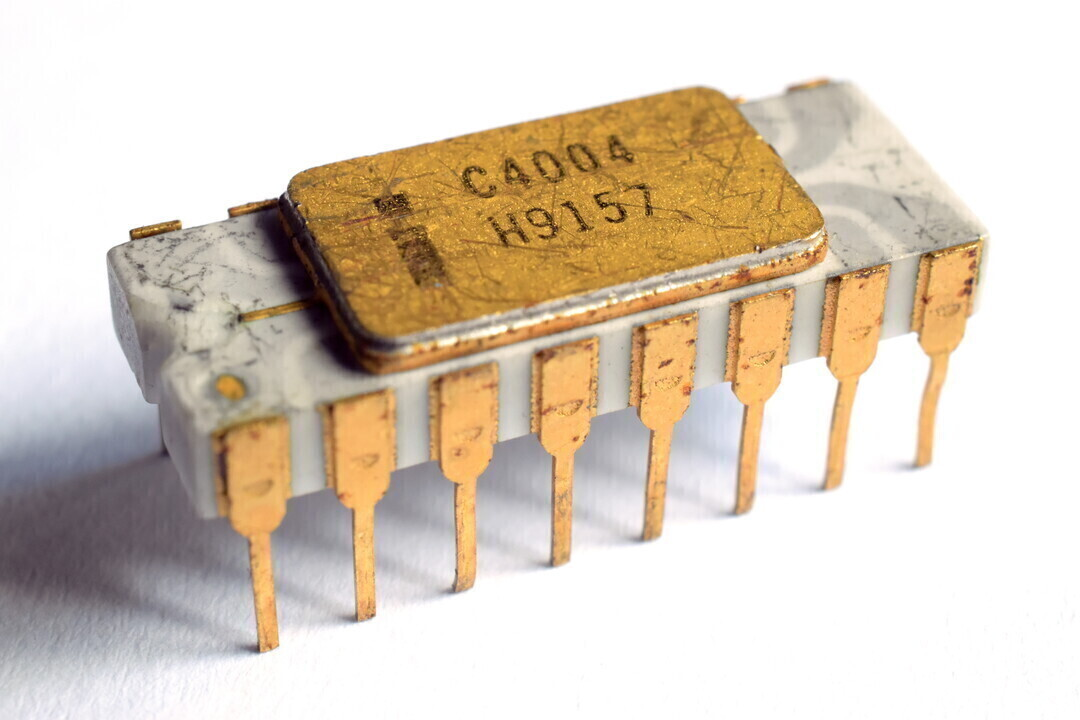
\includegraphics[height=0.5\textheight]{img/intelC4004.jpg}
    \captionsetup{textfont=tiny,labelformat=empty}
    \caption{\ccbysa\cite{intelC4004}}
\end{figure}

\end{frame}

\begin{frame}

\frametitle{Cuarta generación}
\framesubtitle{AMD Ryzen 9 3900X (2019)}

\begin{itemize}
    \item $9\,890\,000\,000$ transistores.
    \item Varios núcleos de procesamiento en un solo componente.
\end{itemize}

\begin{figure}
    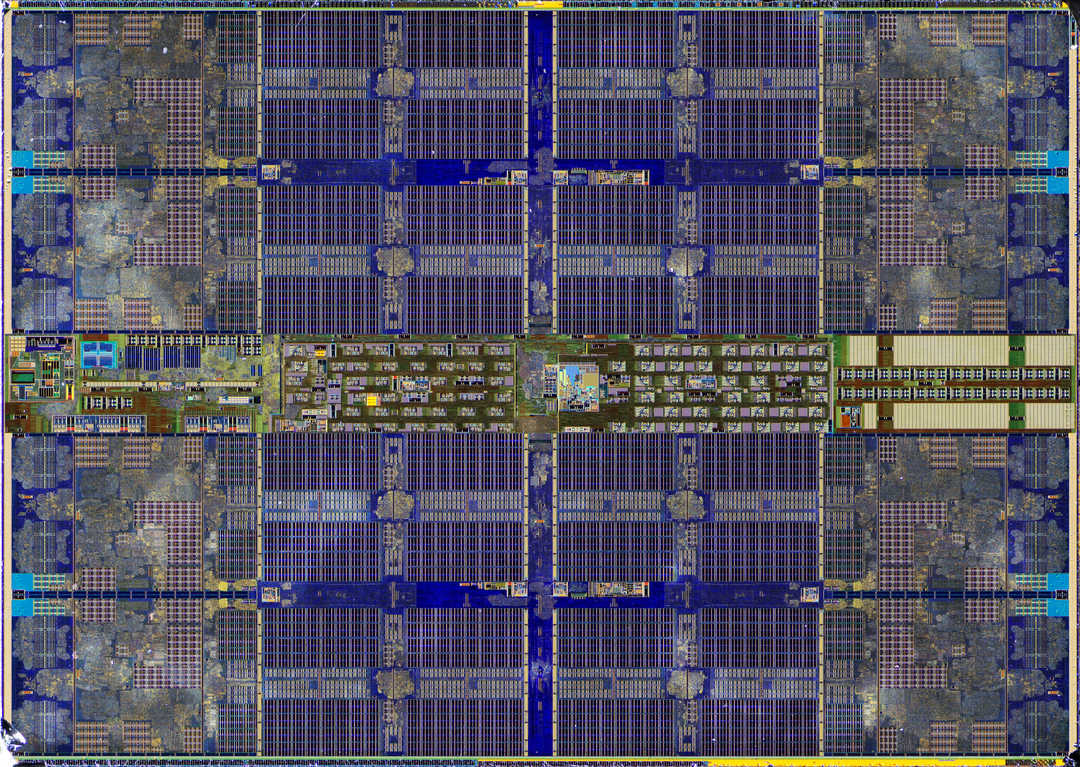
\includegraphics[height=0.75\textheight]{img/amd.jpg}
    \captionsetup{textfont=tiny,labelformat=empty}
    \caption{}
\end{figure}

\end{frame}

\begin{frame}

\frametitle{Cuarta generación}
\framesubtitle{AMD Ryzen 9 3900X (2019)}

\begin{figure}
    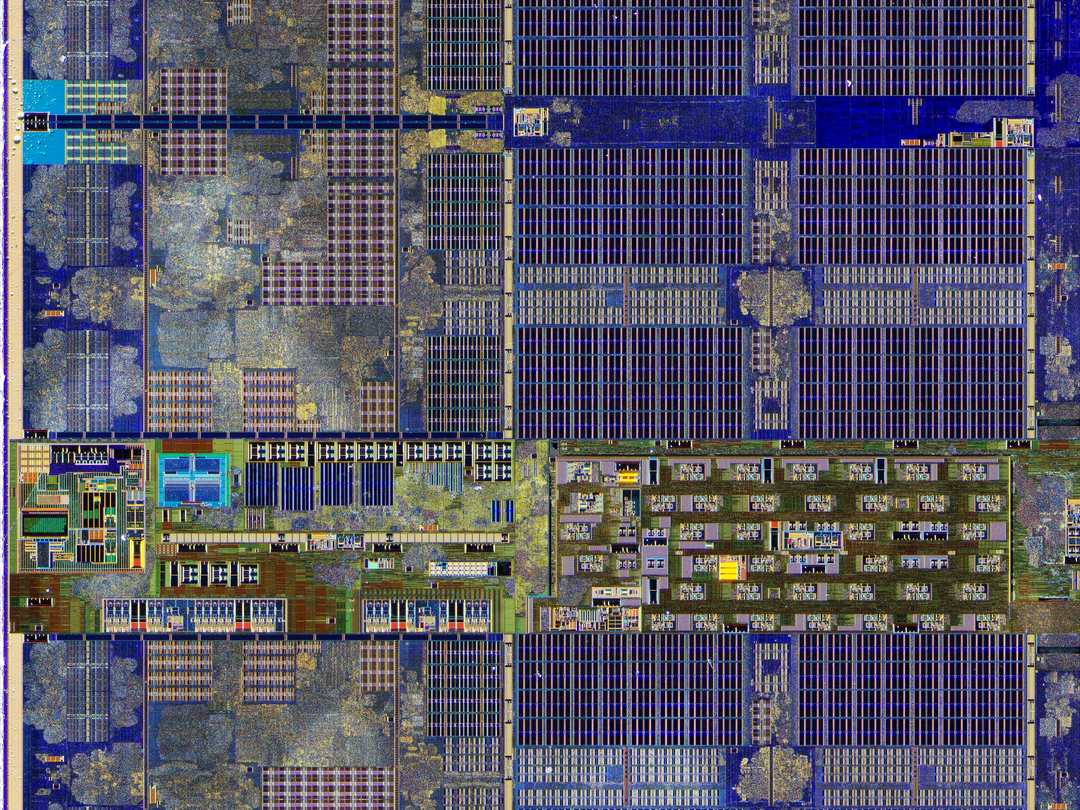
\includegraphics[height=0.90\textheight]{img/amd_zoom.jpg}
    \captionsetup{textfont=tiny,labelformat=empty}
    \caption{}
\end{figure}

\end{frame}

\begin{frame}

    \frametitle{Finalizando}

\begin{enumerate}

    \setcounter{enumi}{-1}

    \item Antecedentes históricos.

    \item Primera generación: válvulas de vacío.

    \item Segunda generación: Transistores.

    \item Tercera generación: Circuitos integrados.

    \item Cuarta generación: Integración a gran escala.

\end{enumerate}

\end{frame}

\begin{frame}

\title{¿Consultas?}
\maketitle

\end{frame}

\begin{frame}%[allowframebreaks]

\frametitle{Atribuciones}

\bibliographystyle{abbrv}
\setbeamertemplate{bibliography item}{\insertbiblabel}
\tiny
\bibliography{refimg}
\end{frame}
%\setcounter{page}{130}

\end{document}
